\documentclass[../main.tex]{subfiles}
\begin{document}
\chapter{2025-2026学年微积分（B）（下）期中考试}

\section{基本计算题(每小题 6 分，共 60 分)}
\begin{enumerate}
    \item 已知向量$\boldsymbol{a}=(2,-1,2)$，$\boldsymbol{b}=(-1,2,-2)$，又向量$\boldsymbol{c}$在$\boldsymbol{a},\boldsymbol{b}$的夹角（在$0$与$\pi$之间）的平分线上，且$|\boldsymbol{c}|=6\sqrt2$，求向量$\boldsymbol{c}$.
          \vspace{9em}

    \item 求过直线
          \(
          L:\begin{cases}
              x+2z+1=0, \\
              x-y-z+1=0
          \end{cases}
          \)
          且与平面$\pi:x+y+2z-4=0$夹角为$\dfrac{\pi}{3}$的平面方程.
          \vspace{10em}

    \item 求曲线
          \(
          \begin{cases}
              2x^2+y^2+z^2=45, \\
              x^2+2y^2=z
          \end{cases}
          \)
          在点$M(-2,1,6)$的切线和法平面方程.
          \vspace{10em}

    \item 设函数
          \(
          f(x,y)=\int_0^{xy}\mathrm{e}^{-t^2}\,\mathrm{d}t+\ln\sqrt{x^2+y^2},
          \)
          求$\mathrm{d}f|_{(1,2)}$.
          \vspace{9em}

    \item 设函数$z=f\left(x^2+y,\dfrac{x}{y}\right)$，其中$f(u,v)$具有二阶连续偏导数，求$\dfrac{\partial^2z}{\partial x\partial y}$.
          \vspace{10em}

    \item 设函数$f(x,y)=2x^2+ax+xy^2+2y$在$(1,-1)$处取得极值，求常数$a$，并确定极值类型.
          \vspace{9em}

    \item 计算二次积分
          \(
          I=\int_0^1\mathrm{d}y\int_{\frac{y}{2}}^y\sin\frac{\pi y}{x}\,\mathrm{d}x
          +\int_1^2\mathrm{d}y\int_{\frac{y}{2}}^1\sin\frac{\pi y}{x}\,\mathrm{d}x.
          \)
          \vspace{10em}

    \item 设$u=f(x,y,z)$，$\varphi(x^2,\mathrm{e}^y,z)=0$，$y=\sin x$，其中$f,\varphi$都具有一阶连续偏导数，且$\frac{\partial\varphi}{\partial z}\neq0$，求$\dfrac{\mathrm{d}u}{\mathrm{d}x}$.
          \vspace{10em}

    \item 计算积分
          \(
          I=\iint\limits_D |x^2+y^2-2x|\,\mathrm{d}x\,\mathrm{d}y
          \)，其中$D=\{(x,y)\mid x^2+y^2\le4\}$.
          \vspace{10em}

    \item 计算积分
          \(
          I=\iiint\limits_V(y\cos x+z)\,\mathrm{d}x\,\mathrm{d}y\,\mathrm{d}z
          \)，其中$V$由曲面$z=x^2+y^2$和$z=\sqrt{2-x^2-y^2}$所围成.
          \vspace{10em}
\end{enumerate}

\section{综合题(每小题 8 分，共 40 分)}
\begin{enumerate}
    \setcounter{enumi}{10}
    \item 求直线$L:\dfrac{x}{\alpha}=\dfrac{y-\beta}{0}=\dfrac{z}{1}$绕$z$轴旋转而成的曲面方程，并就$\alpha,\beta$（$\alpha,\beta$不同时为零）的值讨论方程表示什么曲面？
          \vspace{12em}

    \item 在椭球面$2x^2+2y^2+z^2=1$上求一点，使函数$f(x,y,z)=x^2+y^2+z^2$在该点处沿方向$\boldsymbol{l}=(1,-1,0)$的方向导数最大，并求出该方向导数.
          \vspace{12em}

    \item 曲面$\Sigma$的方程为$z^5-xz^4+yz^3=1$，平面$\pi$为曲面$\Sigma$在点$P(1,1,1)$处的切平面，直线$L_1$为直线
          \[
              L:\begin{cases}
                  2x+2z+1=0, \\
                  x-y-z+1=0
              \end{cases}
          \]
          在平面$\pi$上的投影直线，求点$P(1,1,1)$到直线$L_1$的距离$d$.
          \vspace{13em}

    \item 设函数
          \[
              f(x,y)=
              \begin{cases}
                  \dfrac{x^3}{x^2+y^2}, & x^2+y^2\ne0, \\[0.6em]
                  0,                    & x^2+y^2=0.
              \end{cases}
          \]
          \begin{enumerate}[label=(\arabic*)]
              \item 求$f_x(x,y),f_y(x,y)$；
              \item 讨论函数$f(x,y)$在点$(0,0)$处的可微性.
          \end{enumerate}
          \vspace{12em}

    \item 设$f(x)$是$[0,+\infty)$上的单调减少的连续函数，试证明：对任意$t\ge0$都成立不等式
          \[
              \iint\limits_D\left(\frac{t^2}{x}-6y\right)f(x)\,\mathrm{d}x\,\mathrm{d}y\ge0,
          \]
          其中$D=\{(x,y)\mid0\le y\le t,\ y\le x\le t\}$.
          \vspace{12em}
\end{enumerate}

\chapter{2025-2026学年微积分（B）（下）期中考试参考答案}
\section{基本计算题(每小题 6 分，共 60 分)}
\begin{enumerate}
    \item \textbf{Solution}. 由
          \[
              |\boldsymbol{a}|=|\boldsymbol{b}|=3
          \]
          可知
          \[
              \boldsymbol{a}^0=\left(\frac23,-\frac13,\frac23\right),\qquad
              \boldsymbol{b}^0=\left(-\frac13,\frac23,-\frac23\right).
          \]
          因而夹角内角平分线方向可取
          \[
              \boldsymbol{d}=\boldsymbol{a}^0+\boldsymbol{b}^0=\frac13(1,1,0).
          \]
          单位方向为
          \[
              \boldsymbol{d}^0=\frac{1}{\sqrt2}(1,1,0).
          \]
          又$|\boldsymbol{c}|=6\sqrt2$，故
          \[
              \boldsymbol{c}=6\sqrt2\,\boldsymbol{d}^0=(6,6,0).
          \]

    \item \textbf{Solution}. 显然$x+2z+1=0$与平面$\pi$的夹角不为$\frac{\pi}{3}$，因此可设过$L$的平面束方程为
          \[
              x+2z+1+\lambda(x-y-z+1)=0,
          \]
          其法向量为
          \[
              \boldsymbol{n}_1=(\lambda+1,-\lambda,2-\lambda).
          \]
          平面$\pi$的法向量为$\boldsymbol{n}_2=(1,1,2)$. 由两平面夹角为$\frac{\pi}{3}$，得
          \[
              \frac{|5-2\lambda|}{\sqrt6\sqrt{3\lambda^2-2\lambda+5}}=\frac12.
          \]
          化简得
          \[
              \lambda^2+34\lambda-35=0.
          \]
          所以$\lambda=1$或$\lambda=-35$，代入平面束，得所求平面为
          \[
              2x-y+z+2=0\quad\text{或}\quad 34x-35y-37z+34=0.
          \]

    \item \textbf{Solution}. 令$F=2x^2+y^2+z^2-45$，$G=x^2+2y^2-z$，则
          \[
              \nabla F|_{(-2,1,6)}=(-8,2,12),\qquad
              \nabla G|_{(-2,1,6)}=(-4,4,-1).
          \]
          因而切线方向为
          \[
              \nabla F\times\nabla G=(-50,-56,-24),
          \]
          取切向量$\boldsymbol{\tau} = (25,28,12)$，故切线方程为
          \[
              \frac{x+2}{25}=\frac{y-1}{28}=\frac{z-6}{12}.
          \]
          法平面方程为$25(x+2)+28(y-1)+12(z-6)=0$，即
          \[
              25x+28y+12z-50=0.
          \]

    \item \textbf{Solution}. 由
          \[
              f_x=y\mathrm{e}^{-x^2y^2}+\frac{x}{x^2+y^2},\qquad
              f_y=x\mathrm{e}^{-x^2y^2}+\frac{y}{x^2+y^2},
          \]
          且$f_x,f_y$在$(1,2)$处连续，故$f$在$(1,2)$处可微. 又
          \[
              f_x(1,2)=2\mathrm{e}^{-4}+\frac15,\qquad
              f_y(1,2)=\mathrm{e}^{-4}+\frac25.
          \]
          因此
          \[
              \mathrm{d}f|_{(1,2)}=\left(2\mathrm{e}^{-4}+\frac15\right)\mathrm{d}x+
              \left(\mathrm{e}^{-4}+\frac25\right)\mathrm{d}y.
          \]

    \item \textbf{Solution}. 记
          \[
              u=x^2+y,\qquad v=\frac{x}{y}.
          \]
          则
          \[
              \frac{\partial z}{\partial x}=f_1'u_x'+f_2'v_x'=2xf_1'+\frac1y f_2'.
          \]
          再对$y$求偏导，得
          \[
              \begin{aligned}
                  \frac{\partial^2 z}{\partial x\partial y}= {} & 2x\left(f''_{11}+f''_{12}\cdot\left(-\frac{x}{y^2}\right)\right)-\frac{1}{y^2}f_2'+\frac{1}{y}\left(f''_{21}+f''_{22}\cdot\left(-\frac{x}{y^2}\right)\right) \\
                  = {} & 2xf''_{11}+\frac{y-2x^2}{y^2}f''_{12}-\frac1{y^2}f_2'-\frac{x}{y^3}f''_{22},
              \end{aligned}
          \]

    \item \textbf{Solution}. 因
          \[
              f_x=4x+a+y^2,\qquad f_y=2xy+2,
          \]
          而$f$在$(1,-1)$处取得极值，所以
          \[
              f_x(1,-1)=0,\qquad f_y(1,-1)=0.
          \]
          解得
          \[
              a=-5.
          \]
          此时
          \[
              A=f_{xx}=4,\qquad B=f_{xy}=2y,\qquad C=f_{yy}=2x,
          \]
          在$(1,-1)$处
          \[
              AC-B^2=4\cdot2-(-2)^2=4>0,\qquad A>0.
          \]
          故$f(x,y)$在$(1,-1)$处取得极小值.

    \item \textbf{Solution}.

          \noindent\begin{minipage}[c]{0.58\textwidth}
              由题意绘制积分区域$D$如图所示，可以改写为
              \[
                  D:0\le x\le1,\qquad x\le y\le2x.
              \]
              因而
              \[
                  \begin{aligned}
                      I= {} & \int_0^1\mathrm{d}x\int_x^{2x}\sin\frac{\pi y}{x}\,\mathrm{d}y                 \\
                      = {} & \int_0^1\left[-\frac{x}{\pi}\cos\frac{\pi y}{x}\right]_{y=x}^{2x}\,\mathrm{d}x \\
                      = {} & -\frac{2}{\pi}\int_0^1x\,\mathrm{d}x=-\frac1\pi.
                  \end{aligned}
              \]
          \end{minipage}\hfill
          \begin{minipage}[c]{0.30\textwidth}
              \centering
              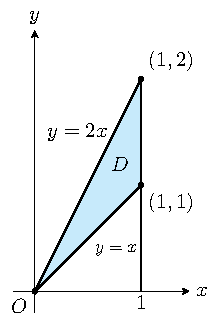
\includegraphics[width=3.6cm]{2026x-figure1.pdf}
          \end{minipage}

    \item \textbf{Solution}. 对方程组
          $\begin{cases}
                  \varphi(x^2,\mathrm{e}^y,z)=0, \\
                  y=\sin x
              \end{cases}$两边关于$x$求导，得
          \(
          \begin{cases}
              2x\varphi_1+\mathrm{e}^y\varphi_2\frac{\mathrm{d}y}{\mathrm{d}x}+
              \varphi_3\frac{\mathrm{d}z}{\mathrm{d}x}=0, \\
              \frac{\mathrm{d}y}{\mathrm{d}x}=\cos x.
          \end{cases}
          \)

          解得
          \[
              \frac{\mathrm{d}z}{\mathrm{d}x}
              =-\frac{2x\varphi_1+\mathrm{e}^y\cos x\,\varphi_2}{\varphi_3}.
          \]
          再对$u=f(x,y,z)$两边关于$x$求导，得
          \[
              \frac{\mathrm{d}u}{\mathrm{d}x}
              =f_1'+\cos x\,f_2'
              -\frac{2x\varphi_1+\mathrm{e}^y\cos x\,\varphi_2}{\varphi_3}f_3'.
          \]

    \item \textbf{Solution}.

          \noindent\begin{minipage}[c]{0.49\textwidth}
              记
              \[
                  f=x^2+y^2-2x.
              \]
              令
              \[
                  D_1:x^2+y^2\le2x,\qquad D_2=D\setminus D_1.
              \]
              则$f\le0$于$D_1$，$f>0$于$D_2$，故
              \[
                  I=-2\iint\limits_{D_1}f\,\mathrm{d}x\,\mathrm{d}y+\iint\limits_D f\,\mathrm{d}x\,\mathrm{d}y.
              \]
              用极坐标代换，
              \[
                  \begin{aligned}
                      I= {} & 2\int_{-\frac{\pi}{2}}^{\frac{\pi}{2}}\mathrm{d}\theta\int_0^{2\cos\theta}(2r\cos\theta-r^2)r\,\mathrm{d}r                              \\
                            & +\int_0^{2\pi}\mathrm{d}\theta\int_0^2(r^2-2r\cos\theta)r\,\mathrm{d}r                                                                  \\
                      = {}  & \frac{16}{3}\int_0^{\frac{\pi}{2}}\cos^4\theta\,\mathrm{d}\theta+\int_{0}^{2\pi}\left(4-\frac{16}{3}\cos\theta\right)\,\mathrm{d}\theta \\
                      = {}  & \frac{16}{3}\cdot \frac{3}{4}\cdot \frac{1}{2} \cdot \frac{\pi}{2} + 8\pi = 9\pi.
                  \end{aligned}
              \]
          \end{minipage}\hfill
          \begin{minipage}[c]{0.44\textwidth}
              \centering
              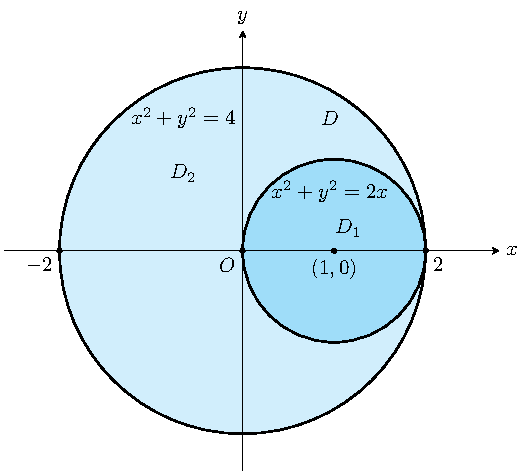
\includegraphics[width=6.2cm]{2026x-figure2.pdf}
          \end{minipage}

    \item \textbf{Solution}. 由对称性可知
          \[
              \iiint\limits_Vy\cos x\,\mathrm{d}x\,\mathrm{d}y\,\mathrm{d}z=0.
          \]
          联立两曲面方程可得交线在$xOy$平面上的投影为
          \[
              x^2+y^2=1.
          \]
          因而
          \[
              I=\iiint\limits_V z\,\mathrm{d}x\,\mathrm{d}y\,\mathrm{d}z
              =\iint\limits_{x^2+y^2\le1}\mathrm{d}x\,\mathrm{d}y
              \int_{x^2+y^2}^{\sqrt{2-x^2-y^2}}z\,\mathrm{d}z.
          \]
          用极坐标代换，
          \[
              \begin{aligned}
                  I= {} & \int_{0}^{2\pi}\,\mathrm{d}\theta\int_{0}^{1}r\,\mathrm{d}r\int_{r^2}^{\sqrt{2-r^2}}z\,\mathrm{d}z \\
                  = {}  & \pi\int_0^1(2-r^2-r^4)r\,\mathrm{d}r                                                               \\
                  = {}  & \pi\left.\left(r^2-\frac{1}{4}r^4-\frac{1}{6}r^6\right)\right|_0^1=\frac{7\pi}{12}.
              \end{aligned}
          \]
\end{enumerate}

\section{综合题(每小题 8 分，共 40 分)}
\begin{enumerate}
    \setcounter{enumi}{10}
    \item \textbf{Solution}. 将直线写成参数方程$\begin{cases}
                  x=\alpha t, \\
                  y=\beta,    \\
                  z=t
              \end{cases}$，直线在绕$z$轴旋转的过程中，对应点到$z$轴的距离不变.

          设$M_0(x_0,y_0,z_0)$为$L$上的点，绕$z$轴旋转到点$M(x,y,z)$，则有
          \[
              \begin{cases}
                  x^2+y^2=x_0^2+y_0^2 = \alpha^2t^2+\beta^2, \\
                  z=z_0=t.
              \end{cases}
          \]
          消去$t$得旋转曲面方程
          \[
              x^2+y^2-\alpha^2z^2=\beta^2.
          \]

          当$\alpha=0$，$\beta\neq0$时，方程为$x^2+y^2=\beta^2$，表示圆柱面；

          当$\alpha\neq0$，$\beta=0$时，方程为$x^2+y^2=\alpha^2z^2$，表示圆锥面；

          当$\alpha\neq0$，$\beta\neq0$时，方程为$\frac{x^2+y^2}{\beta^2}-\frac{\alpha^2z^2}{\beta^2}=1$，表示单叶双曲面.

    \item \textbf{Solution}. 方向$\boldsymbol{l}$的单位向量为
          \[
              \boldsymbol{l}^0=\frac{1}{\sqrt{2}}\left(1,-1,0\right).
          \]
          设椭球面上一点为$(a,b,c)$，则
          \[
              2a^2+2b^2+c^2=1.
          \]
          因
          \[
              \nabla f(a,b,c)=(2a,2b,2c),
          \]
          所以方向导数为
          \[
              \frac{\partial f}{\partial \boldsymbol{l}}\bigg|_{(a,b,c)}
              =\nabla f(a,b,c)\cdot\boldsymbol{l}^0=\sqrt2(a-b).
          \]
          问题转化为在约束$2a^2+2b^2+c^2=1$下求$\sqrt2(a-b)$的最大值.

          用 Lagrange 乘数法，设$L(a,b,c,\lambda)=\sqrt2(a-b)+\lambda(2a^2+2b^2+c^2-1)$，令$\nabla L=\mathbf{0}$，得
          \[
              \begin{cases}
                  \sqrt{2}+4\lambda a=0,  \\
                  -\sqrt{2}+4\lambda b=0, \\
                  2\lambda c=0,           \\
                  2a^2+2b^2+c^2=1.
              \end{cases}
          \]
          解得驻点为$M_1\left(\frac{1}{2},-\frac{1}{2},0\right)$或$M_2\left(-\frac{1}{2},\frac{1}{2},0\right)$.

          计算$\left.\frac{\partial f}{\partial \boldsymbol{l}}\right|_{M_1}=\sqrt{2}\left(\frac{1}{2}+\frac{1}{2}\right)=\sqrt{2}$，$\left.\frac{\partial f}{\partial \boldsymbol{l}}\right|_{M_2}=\sqrt{2}\left(-\frac{1}{2}-\frac{1}{2}\right)=-\sqrt{2}$，

          所以在椭球面上的点$\left(\frac{1}{2},-\frac{1}{2},0\right)$处函数$f$沿方向$\boldsymbol{l}$的方向导数最大，最大值为$\sqrt{2}$.

    \item \textbf{Solution}. 令
          \[
              F(x,y,z)=z^5-xz^4+yz^3-1.
          \]
          则
          \[
              \nabla F(1,1,1)=(-1,1,4).
          \]
          故切平面$\pi$为$-(x-1)+(y-1)+4(z-1)=0$，即
          \[
              x-y-4z+4=0.
          \]
          设过直线$L$的平面束方程为
          \[
              2x+2z+1+\lambda(x-y-z+1)=0.
          \]
          令该平面垂直于$\pi$，可得$(\lambda+2,-\lambda,-\lambda+2)\cdot(-1,1,4)=0$，解得$\lambda=1$，从而平面为
          \[
              3x-y+z+2=0.
          \]
          所以投影直线$L_1$为
          \[
              \begin{cases}
                  x-y-4z+4=0, \\
                  3x-y+z+2=0.
              \end{cases}
          \]
          取$L_1$上一点$P_1(1,5,0)$，则$\overrightarrow{P_1P}=(0,-4,1)$，又直线的方向向量可取为
          \[
              \boldsymbol{s}_1=(1,-1,4)\times(3,-1,1)=(-5,-13,2).
          \]
          故
          \[
              d=\frac{|\overrightarrow{P_1P}\times\boldsymbol{s}_1|}{|\boldsymbol{s}_1|}
              =\frac{5\sqrt{1+1+16}}{\sqrt{25+169+4}}=\frac{5\sqrt{11}}{11}.
          \]

    \item \textbf{Solution}. 当$(x,y)\ne(0,0)$时，
          \[
              f_x(x,y)=\frac{x^2(x^2+3y^2)}{(x^2+y^2)^2},\qquad
              f_y(x,y)=-\frac{2x^3y}{(x^2+y^2)^2}.
          \]
          又
          \[
              f(x,0)=x,\qquad f(0,y)=0,
          \]
          所以
          \[
              f_x(0,0)=1,\qquad f_y(0,0)=0.
          \]
          因而
          \[
              f_x(x,y)=
              \begin{cases}
                  \dfrac{x^2(x^2+3y^2)}{(x^2+y^2)^2}, & x^2+y^2\ne0, \\[0.6em]
                  1,                                  & x^2+y^2=0,
              \end{cases}
          \]
          \[
              f_y(x,y)=
              \begin{cases}
                  -\dfrac{2x^3y}{(x^2+y^2)^2}, & x^2+y^2\ne0, \\[0.6em]
                  0,                           & x^2+y^2=0.
              \end{cases}
          \]
          下面讨论函数$f(x,y)$在点$(0,0)$处的可微性. 因为
          \[
              f(x,y)-f(0,0)-f_x(0,0)x-f_y(0,0)y
              =\frac{x^3}{x^2+y^2}-x=-\frac{xy^2}{x^2+y^2},
          \]
          所以
          \[
              \frac{f(x,y)-f(0,0)-f_x(0,0)x-f_y(0,0)y}{\sqrt{x^2+y^2}}
              =-\frac{xy^2}{(x^2+y^2)^{\frac{3}{2}}}.
          \]
          问题转化为判断$\lim_{\substack{x\to0 \\ y\to0}}\frac{xy^2}{(x^2+y^2)^{\frac{3}{2}}}$是否为$0$.

          考虑路径$y=x$，由于$\lim_{\substack{x\to0 \\ y=x}}\frac{-xy^2}{(x^2+y^2)^{\frac{3}{2}}}=\lim_{x\to0}\frac{-x^3}{\left(2x^2\right)^{\frac{3}{2}}}=-\frac{1}{2\sqrt{2}}\lim_{x\to0}\frac{x^3}{\left|x^3\right|}$不存在，

          这意味着$\lim_{\substack{x\to0 \\ y\to0}}\frac{f(x,y)-f(0,0)-f_x(0,0)x-f_y(0,0)y}{\sqrt{x^2+y^2}}$不存在，因此函数$f(x,y)$在点$(0,0)$处不可微.

    \item \textbf{Proof}. 交换积分次序可得
          \[
              \iint\limits_D\left(\frac{t^2}{x}-6y\right)f(x)\,\mathrm{d}x\,\mathrm{d}y
              =\int_0^t f(x)\,\mathrm{d}x\int_0^x\left(\frac{t^2}{x}-6y\right)\,\mathrm{d}y.
          \]
          即
          \[
              \iint\limits_D\left(\frac{t^2}{x}-6y\right)f(x)\,\mathrm{d}x\,\mathrm{d}y
              =\int_0^t(t^2-3x^2)f(x)\,\mathrm{d}x.
          \]
          记
          \[
              F(t)=\int_0^t(t^2-3x^2)f(x)\,\mathrm{d}x.
          \]
          则
          \[
              F'(t)=2t\int_0^t f(x)\,\mathrm{d}x+t^2f(t)-3t^2f(t)
              =2t\int_0^t(f(x)-f(t))\,\mathrm{d}x.
          \]
          由于$f$单调减少，当$0\le x\le t$时，$f(x)\ge f(t)$，故$t\ge0$时$F'(t)\ge0$. 又$F(0)=0$，所以$F(t)\ge0$，即
          \[
              \iint\limits_D\left(\frac{t^2}{x}-6y\right)f(x)\,\mathrm{d}x\,\mathrm{d}y\ge0.
          \]
\end{enumerate}
\end{document}
